\chapter{Redesign and Implementation}
Large parts of the system were rewritten and improved upon such as the GUI and sensory manager. The benefits resulted in simplification of use at the higher level (such as implementing storyboards) and a better representation of the causes of sensory overloads.

Selecting actions to interact with objects is now less intrusive. Prior a menu would pop up and prompt the user to make a selection with their mouse which will now only happen if there are multiple options. With the removal of description boxes, thoughts are now displayed at the bottom of the screen when to user is looking at a specific object.

Performance issues which were not previously too severe now required direct attention. The game requires a frame rate of 30fps(frame per second) or above in order to be fluent and played without lag. Scenes are required to have a maximum of 100k vertices(from models) with an average of 10-50k. Each pointlight(which is a light the user can turn on/off) used requires the scene to be rendered again and so the number of vertices double with each point light used. Thus, even when keeping within the limits, the amount of lights being used in the game was pushing it to well over a million and the frame frequently dropped below the desired threshold. This was occurring on a computer with a decent processor and graphics card, thus playing on a low-powered machine would not be a good experience.  

Having originally taken a large amount of models from other websites and using programs such as sketchup to aid quicker development, these were found to be inefficient at runtime. Efforts therefore were spent on re-learning the details of blender and what is required to make lightweight game models. 

Where previously the entire house modelled and then imported, the solution to the above problem was to split the house into individual rooms/scenes. When the user then clicks a door, the required scene is loaded very quickly. This approach allows for inclusion of more detailed models within each scene as each scene is only a small room. The problems to performance caused by point lights is then reduced as it is only rendering a single room again, not the entire house. 

Further benefits from compartmentalising the house into rooms arose for dealing with the model pipeline. It became much easier to create individual models and link them into the scene, so if the model needed to be edited it could be without requiring the pain of reimporting and fixing textures or materials. 

The result of the restructure meant the FPS improved tenfold, from an average of 30fps to 200-400fps. If any objects were found to be creating problems from being too detailed or not textures properly, they could be removed without impacting on the rest of the scene.

\section{Storyboards}
Following the prototype which had little story or goals, a more in-depth story and set of tasks were created. The user will play as an example "Day in the life of a child with autism". This will be split up into several "Missions"(tasks). The initial story was developed with consultation from two individuals; One was an adult with autism whom has a child with autism and the second was a 12-year old with autism.

\subsection*{Mission 1: Complete morning routine}
Complete your morning routine in the designated time(the more out of time, the more contentment drops). Player starts in the bedroom which is a designated safe place/sensory room. 

Routine to complete: eat breakfast, brush teeth, get dressed.

\textbf{Game points}
\begin{enumerate}
\item User progresses to the kitchen for breakfast. Possibly use a particle emitter to make lots of ‘germs’ appear in the kitchen.
\item After breakfast the user must go to the bathroom and brush teeth which reduces contentment due to bristles harsh texture. Noise from the toilet scares and prompts the the user to run out of bathroom into the hallway.
\item The lamp in the hallway however has now been turned on and the hallway looks different, the light causes discomfort. The character freezes and the player is unable to move forward but can move backwards. The user can turn the lamp off at the plug but at this point may not be aware of this. If a meltdown occurs, start back in the bedroom with a message that you can turn the lamp off at the plug. When the user returns from a meltdown contentment will not be at its maximum.
\item User clicks wardrobe to get dressed, information displays explaining that certain clothing can feel extremely uncomfortable for someone with autism and can be compared to sandpaper.
\item Morning ends in the bedroom with player not wanting to leave (the plug to the lamp is away from the bedroom so the player has to pass lamp to turn it off) and trying to play/recuperate. Parent then comes in and says “Cmon, we need to go out!”.
\item Child has a meltdown, thoughts flood the screen with fears and anxieties. Where are we going? Are we taking the car? When will I be back? Stomach hurts, stomach hurts - words become even more jumbled. They weren't warned and thought they could replenish energy levels in their room, the change means the rest of the day could be faced with countless unprepared fears.
\end{enumerate}

\subsection*{Mission 2: Afternoon, find out the cause of stomach pain}
Mission is to find out why the characters stomach may be hurting which also gives the user a chance to explore. Contentment slowly drops until the solution is found. Reasons for the pain could be:

\begin{itemize}
\item Hunger/Thirsty
\item Upset stomach or cramps
\item Toilet?
\end{itemize}

The user will be expected to attempt all of the above(the final one the user finds will always be the cause). During the above the door bell will unexpectedly ring and a new character will enter, the parent's friend. The friend was meant to be meeting you both out but due to the earlier meltdown has come to the house instead. Mum tried to explain in advance but words weren't making sense. The person looks like a stranger and can't be recognised and contentment reduces(touch sensitivity occurring from this stranger?). 

\subsection*{Mission 3: Evening, get to bed}
Mission pops up that it is time to go to bed but mum stops you and says you can continue playing. Parent then approaches after an unknown amount of time and informs you to go to bed. Meltdown occurs as it's not the exact time and the characters bedtime routine has been broken.

\section{House design}
Following a need to compartmentalise the previous house environment as a solution to performance issues, a new and more structured plan of the house was created. The game description column of the table is information the user will see when they interact with the object and will be displayed as "thoughts":

\begin{table}[H]
    \begin{tabular}{| p{2cm} | p{2cm} | p{3cm} | p{3cm} | p{4cm} |}
    \hline
    Room & Object & Action & Game description & Effects                                                                  \\
    \hline
    \hline
     Bedroom & Dinosaur & Play: Increases contentment by playing with it & People with autism have special interests. These special interests help with xyz &                   \\
    \hline
    & Touchside lamp & On/off: slowly adjust the light so it does not turn off rapidly. Contentment goes up when light turned off slowly & & If the light goes off too quickly, contentment increases slightly but then rapidly declines. Room looks strange/scary as eyes not yet adjusted    \\
    \hline
    & Collections of items & & Explains that children with autism have an obsession/need to complete collections &  \\
    \hline
    & Wardrobe & Get dressed & Explanation that clothes can be compared to feeling sandpaper & Contentment reduces  \\
    \hline
   & Spinny object & & & All noise blurs out. Contentment increases \\
    \hline 
    Upstairs hallway & Fluorescent light & Turn on/off. Same effect as bedside lamp & Explanation about fluorescent lights. Effects are like ten camera flashes in your eyes & Lights flicker and cause a 'high' effect on sensory system. Disorientation if exposed too long. \\
    \hline
    & Mirror & "Look into" & I don't recognise this person. Not normal having yourself peering back at you & Causes dizzy/disorientation because it is an odd image to see. \\
    \hline
    & Wallpaper & & & Make wallpaper material move and cause dizziness/sensory effects. \\
    \hline
        Downstairs hallway & Flowers & & & They can either smell good or bad. \\
    \hline
    & Door bell & Automated: on/off & Nicer sound could prompt the user to play with it. Can cause anxiety as doorbell may mean unwanted people in safe space & If player rings it is fine. If another person, causes problems.
    \\
    \hline
    \end{tabular}
\end{table}

\begin{table}[H]
    \begin{tabular}{| p{2cm} | p{2cm} | p{3cm} | p{3cm} | p{4cm} | }
    \hline
    Room & Object & Action & Game Description & Effects                                                                  \\
    \hline
    \hline
        Kitchen & Washing machine & Turn on/off & Could become transfixed with spinning nature & Noisy, need to move away. \\
    \hline
    & Kitchen sides & & Particle emitters to show germs/smells & Reduces contentment \\
    \hline
    & Frying pan & & & Sounds, smells, contentment reduction \\
    \hline
    Living room & TV & Turn on/off & Description indicating that child may think items on TV are identical to what they will get & TV being too loud may hurt. \\
    \hline
    & Hoover & & Description indicating that the noise from Hoovers can be painful & Sensory problems when turned on \\
    \hline
    Bathroom & Bath & Empty bath & & Horrible/scary noises. \\
    \hline
    & Tooth brush & & & Brushing teeth causes contentment to reduce. \\
    \hline
    \end{tabular}
\end{table}

In addition to this, light switches were added as prior the user would have to click on the object itself. A distance measure was added to actions to make sure that users were close enough to the objects to interact with them. This was necessary for the morning routine and unexpected light turning on; otherwise users would be able to turn it off at a distance which is unrealistic and makes it easy to avoid.

\subsection{Sounds}
One of the tasks in moving from the prototype to the first version was to create a more immersive environment, the addition sound was felt to promote this.

Research was first conducted to find which sounds may be problematic for someone with autism, this was a difficult process involving guess-work and then requesting feedback. It was challenging to put oneself into the shoes of someone with autism and identify what sounds around the house would cause issues. The solution came by finding adults an autism whom would be willing to record sounds around their house that they personally find troublesome. This gave far more indication than words. Previously for example "I find the bath a problem" was misinterpreted as it was thought the noise of the bath plug when pulled that was causing issues, but for one adult it was actually the running of the bath itself in addition the the plug.

Sounds recorded were:

\begin{enumerate}
\item Hoover - Planned
\item Humming from the fridge - Unplanned(recording not great)
\item Light switch turning on
\item Kitchen light sounds(it is a fluorescent light)
\item Washing machine - Planned
\item Dog barking - Unplanned
\item Toilet flushing - Planned
\item Dog drinking - Unplanned
\item Sounds of walking up stairs - Unplanned. Replaced with general footstep noises
\item Brushing teeth - Planned
\item Doorbell - Planned
\item Drinking - Planned
\item Heating/boiler - Unplanned
\item Filling up glass - Planned
\item TV noise - Planned
\end{enumerate}

By asking someone with autism to record the sounds themselves, it personally gave me an experience of the types of things they hear and thus revealed what I needed to convey rather than using guesswork. Sounds such as the humming from the fridge were never considered until the results of the recordings came. Some of these will not be incorporated into the first version, but left for a later date. 


\subsection{Rewrite of scenes}
Most the the effort in the last few weeks of the semester were spend on re-writing the scene manager and remodelling the house. 

\begin{figure}[H]
\centering
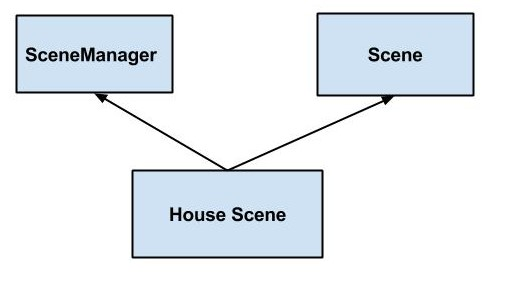
\includegraphics[width=90mm]{images/scenemanager.jpg}
\caption{}
\label{scenemanager}
\end{figure}

SceneManager contains useful tools for the creation, deletion and changing of scenes. The "HomeScene" extends this and contains objects which are all instances of Scene and represent the individual rooms. By extending the SceneManager the HomeScene can listen to events occurring in the game and specify custom ones that are unique for that collection of scenes(or rooms), for example it can specify that doors require changing and loading of different rooms. 

\subsubsection{House implementation}
In addition to remodelling parts of the house a bathroom was created and added along with new actions such as being able to flush the toilet(with sounds to accompany this). Now being able to handle individual objects in rooms allows for easy addition animation, the clock's hands in the room move and will indicate the time of day. Below gives some screen shots of the new environment and it's accompanying frame-rates. 


\begin{figure}[H]
\centering
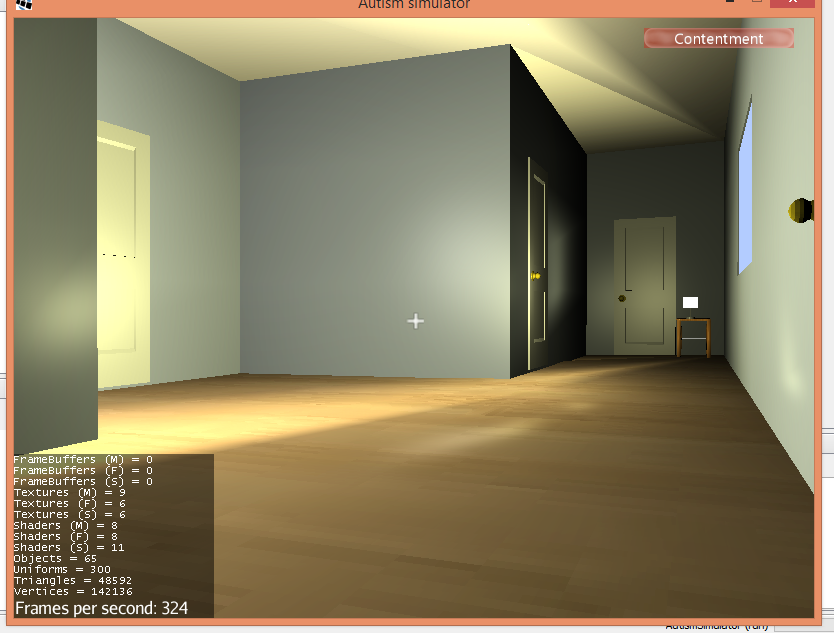
\includegraphics[width=90mm]{images/new_hallway1.png}
\caption{Image of new hallway}
\label{newhallway}
\end{figure}

\begin{figure}[H]
\centering
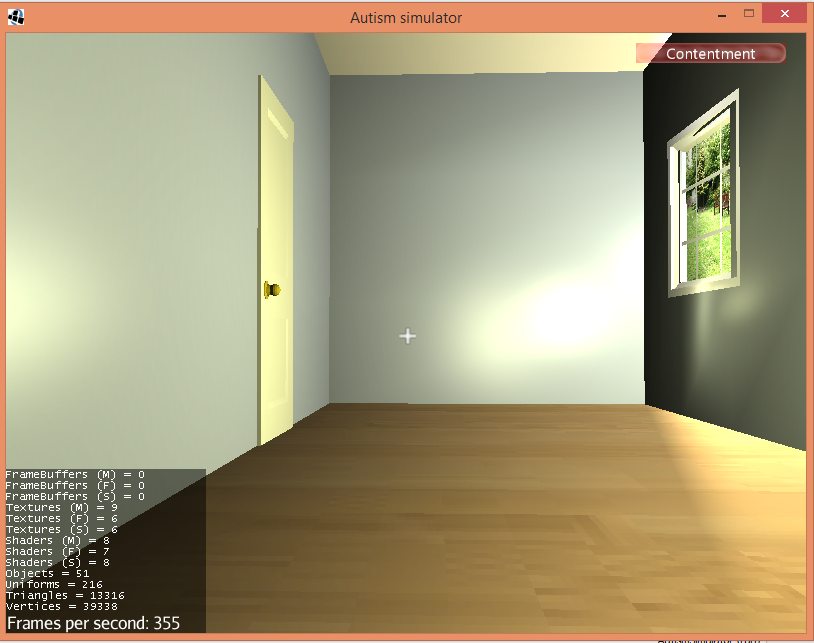
\includegraphics[width=90mm]{images/new_hallway2.png}
\caption{Image of new hallway}
\label{newhallway2}
\end{figure}

\begin{figure}[H]
\centering
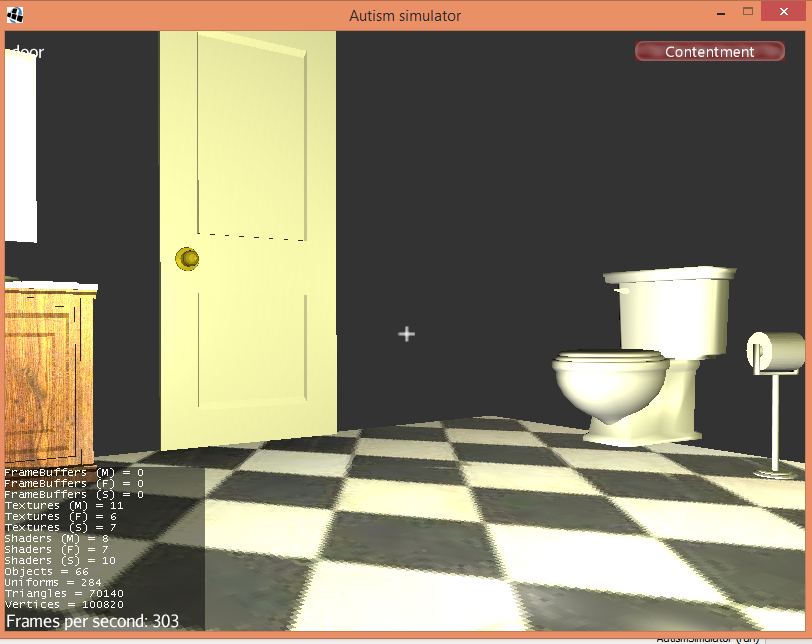
\includegraphics[width=90mm]{images/new_bathroom.png}
\caption{Image of bathroom that was previously missing from the house}
\label{old_house}
\end{figure}

\begin{figure}[H]
\centering
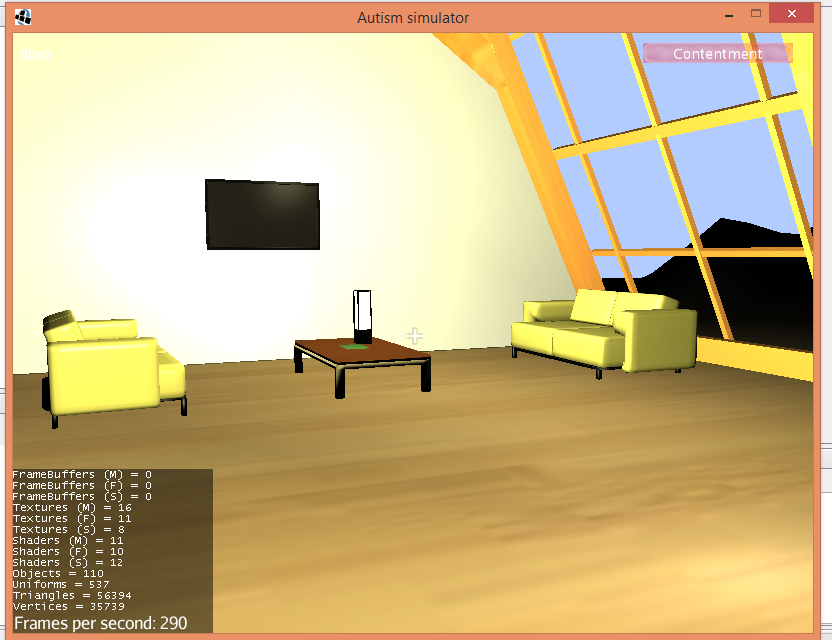
\includegraphics[width=90mm]{images/new_livingroom.png}
\caption{Image of new livingroom}
\label{old_house}
\end{figure}

\subsection{Game state manager}

As the size of the system grew, one of the most important changes was the addition of a game state manager, enabling universal control and monitoring of the overall system. 

The user can now change between "Explore mode"(the user has no tasks and can simply look around the environment) and "Mission mode"(given the tasks or story) without having to restart the simulator. From this came the addition of the start and help screen and ability for the user to pause the game.  

The rest of the system can now request useful information from the GSM such as which mission is currently being run, which scene the player is currently in and what the state of the GUI is (if actions are being displayed, if the user is required to select an option). If the GUI needs to display information(such as selecting actions) it will notify the game state manager which will halt processes that may interfere. Having a central control made other parts of the simulator easier to develop and reuse since each part of the system only needs to worry about which state it is in rather than checking multiple conditions.

\subsection{Sensory System improvements}
Following the feedback on sensory overloads, improvements were required in how sensory overloads occurred rather than what was happening when they did. Previously, objects which could affect the sensory system were put into a Hashable which were then periodically checked for the distance to the player and if in proximity, would affect the sensory system depending on how far the object is. However, all objects would affect the user by the same weight and the effect on contentment would change depending on what threshold of objects were reached (i.e if 2 were in proximity the health reduction would be low, if more than two the reduction would be greater). Filters to mirror sensory overloads would then be applied depending on this level.

\begin{figure}[H]
\centering
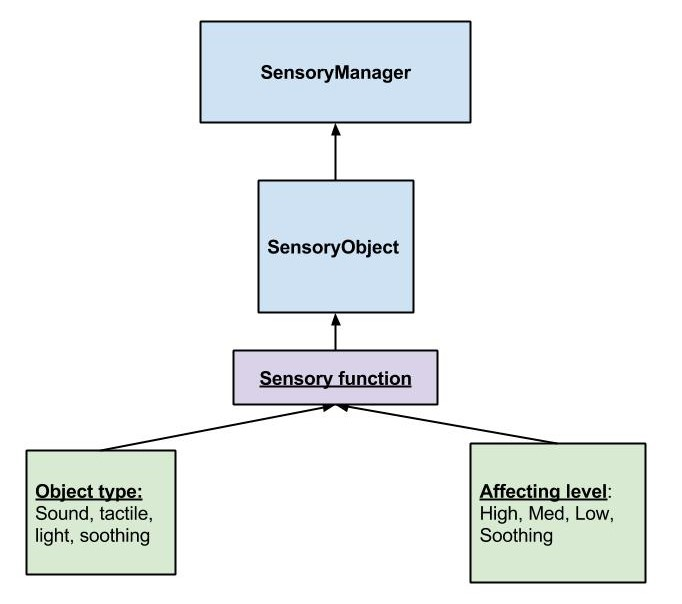
\includegraphics[width=90mm]{images/sensoryobjects.jpg}
\caption{Diagram showing implementation of sensory system}
\label{sensorysystem}
\end{figure}

The new implementation attempts to create a better less fragmented model of how objects affect the player and cause sensory overloads/meltdowns. This approach is more scalable and enables a flexible means to experiment by simply changing parameters, thus helping to address previous issues of meltdowns occurring too quickly.

Each sensory object is given two properties (from the green boxes above) and from this a sensory function is applied and a weight for each object is calculated. The sensory function is simply an exponential: the higher the affecting level the higher the weight returned and if the object is set as a 'soothing object' a negative value will return instead. 

The sensory manager then takes all the weights of the objects that are in proximity and sums them, taking the log of this. If the log is negative there are no objects and contentment replenishes. The result of the summation is then taken away from the players contentment. 

Sounds were the final addition to the simulator. When acting on the toilet it now flushes and the alarm clock in the room rings. Sounds create a more immersive environment and an additional layer for creating sensory overloads(i.e making objects more high-pitched). 